\section{时间离散}
\label{sec:odenum-time-discretization}

连续的解是一条曲线，算法只能交出有限个数。这有限个数应该是什么，怎样一个接一个地产生，又该拿什么标准评价它们？

\paragraph{时间网格与一步更新}
固定初值问题
\begin{equation}
 \dot{\bm{x}}(t)=\bm{f}(t,\bm{x}(t)),\qquad \bm{x}(t_0)=\bm{x}_0,
 \label{eq:odenum-ivp}
\end{equation}
并假定它在有限区间$[t_0,t_0+T]$上有唯一解$\bm{x}(t)$，$\bm{x}(t)\in\mathbb{R}^{n}$。存在、唯一与延拓的条件见第~\ref{chap:ode-existence-continuation}章。

把区间等分成$N$份，步长$h=T/N$，得到\term{时间网格}（time grid）
\begin{equation}
 t_k=t_0+kh,\qquad k=0,1,\ldots,N.
 \label{eq:odenum-grid}
\end{equation}
数值解是一串向量$\bm{x}^{(0)},\bm{x}^{(1)},\ldots,\bm{x}^{(N)}$，其中$\bm{x}^{(k)}$用来近似$\bm{x}(t_k)$。上标带括号表示网格编号，不是导数的阶数。

真解自身满足一个“一步”关系。在$[t_k,t_{k+1}]$上积分方程，得到
\begin{equation}
 \bm{x}(t_{k+1})=\bm{x}(t_k)+\int_{t_k}^{t_{k+1}}\bm{f}(s,\bm{x}(s))\,\mathrm{d}s.
 \label{eq:odenum-integral-step}
\end{equation}
右端的积分依赖这一步内部尚不知道的解，所以不能直接算。本章所有方法都在回答同一件事：只用当前已知的量，怎样近似这个积分。

用流映射的话说，式~\eqref{eq:odenum-integral-step}就是
\[
 \bm{x}(t_{k+1})=\bm{\varphi}_{t_k,t_{k+1}}\bigl(\bm{x}(t_k)\bigr),
\]
其中$\bm{\varphi}_{s,t}(\bm{y})$表示时刻$s$从$\bm{y}$出发的解在时刻$t$的值。流映射一般算不出来，于是用一个可计算的映射代替它。

\begin{definition}[一步方法]
 \label{def:odenum-one-step}
 \term{一步方法}（one-step method）由一族映射$\bm{\Psi}_h(t,\cdot)$给出，步长为$h$时按
 \begin{equation}
  \bm{x}^{(k+1)}=\bm{\Psi}_h\bigl(t_k,\bm{x}^{(k)}\bigr),\qquad k=0,1,\ldots,N-1
  \label{eq:odenum-one-step}
 \end{equation}
 从$\bm{x}^{(0)}$逐步计算。$\bm{\Psi}_h$只依赖当前的$t_k$、$\bm{x}^{(k)}$、步长和右端$\bm{f}$，不依赖更早的网格值。
\end{definition}

\paragraph{连续曲线、网格值与插值结果}
离散之后手里有三种不同的对象，它们很容易被混为一谈。图~\ref{fig:odenum-grid-values}把它们画在一起：蓝线是真解，是我们想知道却拿不到的函数；绿点是网格值，是算法实际产生的全部输出；绿色虚线是把相邻网格值连起来的折线，它是另加的一条规则，并不来自方程。

\begin{BookInlineFigure}
 \centering
 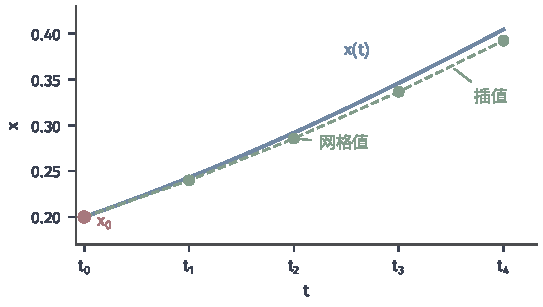
\includegraphics[width=92mm]{figures/06-differential-equations/01-ordinary-differential-equations/matplotlib/odenum-grid-values/figure.pdf}
 \caption{初值问题$\dot{x}=x(1-x)$，$x(0)=0.2$的三种对象。蓝线是真解，红点是初值，绿点是某个一步方法在步长$h=1/4$下给出的网格值，绿色虚线是对网格值作的分段线性插值。}
 \label{fig:odenum-grid-values}
\end{BookInlineFigure}

讨论误差时必须先说清比较的是哪一种对象。本章的误差都指网格点上$\bm{x}^{(k)}$与$\bm{x}(t_k)$的差。

网格点之间的值需要另外的插值规则，插值规则有自己的误差。若方法在网格上很精确，而插值只用分段线性，那么网格点之间的误差由插值决定，只有$h^2$的量级，精确的网格值也就白费了。

\paragraph{三种误差的来源}
数值解离真解有多远，来自三个不同的环节。第一，出发点可能不准：$0.2$在二进制中是无限循环小数，存进计算机时已经有舍入，初值本身也可能来自测量。第二，一步更新只是对式~\eqref{eq:odenum-integral-step}的近似。第三，每一步的运算有舍入误差，隐式方法（第~\ref{sec:odenum-stiff}节）还要加上内部方程没有解到底的误差。

用$\bm{\delta}^{(0)}$记初值误差，用$\bm{\delta}^{(k)}$（$k\geq1$）记第$k$步的计算误差，把实际算出的序列写成
\begin{equation}
 \bm{x}^{(0)}=\bm{x}_0+\bm{\delta}^{(0)},\qquad
 \bm{x}^{(k+1)}=\bm{\Psi}_h\bigl(t_k,\bm{x}^{(k)}\bigr)+\bm{\delta}^{(k+1)}.
 \label{eq:odenum-computed}
\end{equation}
理想算术且初值精确时，所有$\bm{\delta}^{(k)}$都为零。

第二个环节需要单独定义。关键是把出发点放在真解上，这样它只反映更新规则本身的缺陷，不混入以前积累的偏差。

\begin{definition}[局部截断误差与全局误差]
 \label{def:odenum-errors}
 设$\bm{x}(t)$是式~\eqref{eq:odenum-ivp}的解。第$k+1$步的\term{局部截断误差}（local truncation error）是从真解出发走一步与真解的差，
 \begin{equation}
  \bm{\ell}^{(k+1)}=\bm{\Psi}_h\bigl(t_k,\bm{x}(t_k)\bigr)-\bm{x}(t_{k+1}).
  \label{eq:odenum-local-error}
 \end{equation}
 \term{全局误差}（global error）是实际算出的网格值与真解的差，
 \begin{equation}
  \bm{e}^{(k)}=\bm{x}^{(k)}-\bm{x}(t_k).
  \label{eq:odenum-global-error}
 \end{equation}
\end{definition}

注意$\bm{\ell}^{(k+1)}$没有除以步长，它就是一步之内产生的偏差。两种误差的关系可以直接写出来。把式~\eqref{eq:odenum-computed}代入$\bm{e}^{(k+1)}$，再加减$\bm{\Psi}_h(t_k,\bm{x}(t_k))$，得到
\begin{equation}
 \bm{e}^{(k+1)}
 =\underbrace{\bm{\Psi}_h\bigl(t_k,\bm{x}^{(k)}\bigr)-\bm{\Psi}_h\bigl(t_k,\bm{x}(t_k)\bigr)}_{\text{旧误差的传播}}
 +\bm{\ell}^{(k+1)}+\bm{\delta}^{(k+1)}.
 \label{eq:odenum-error-split}
\end{equation}
每步的全局误差等于“上一步误差被更新规则放大或缩小的结果”，加上本步新产生的截断误差和计算误差。图~\ref{fig:odenum-three-errors}画出了这三个环节的位置。

\begin{BookInlineFigure}
 \centering
 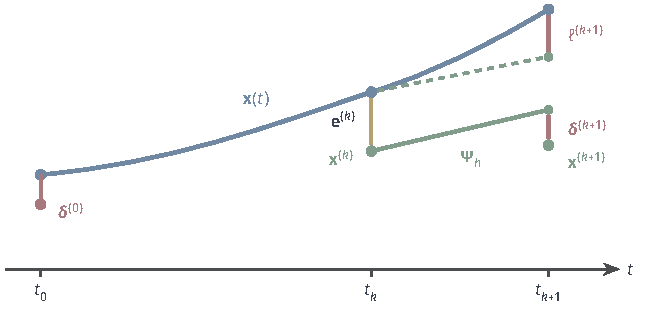
\includegraphics[width=109mm]{figures/06-differential-equations/01-ordinary-differential-equations/tikz/odenum-three-errors/figure.pdf}
 \caption{误差分解的一步。蓝线是真解，红点标出初值误差$\bm{\delta}^{(0)}$；在$t_{k+1}$处，从真解点$\bm{x}(t_k)$按规则$\bm{\Psi}_h$走一步，落点与真解之差是局部截断误差$\bm{\ell}^{(k+1)}$；从算出的$\bm{x}^{(k)}$走一步（绿色），旧误差$\bm{e}^{(k)}$被传播，再叠加计算误差$\bm{\delta}^{(k+1)}$后得到$\bm{x}^{(k+1)}$。}
 \label{fig:odenum-three-errors}
\end{BookInlineFigure}

\paragraph{残差不能代替误差}
既然真解满足方程，一个诱人的检验是把近似解代回方程，看方程满足得好不好。这种检验要分两种情况看。

如果代入的是离散格式本身，得到的永远是零。网格值正是按式~\eqref{eq:odenum-one-step}算出来的，无论$h$多大，它都严格满足自己的递推，所以离散方程的残差不提供任何信息。

如果代入的是连续的插值函数$\tilde{\bm{x}}(t)$，就可以定义\term{残差}（residual）
\[
 \bm{r}(t)=\dot{\tilde{\bm{x}}}(t)-\bm{f}\bigl(t,\tilde{\bm{x}}(t)\bigr).
\]
残差小说明$\tilde{\bm{x}}$是一个“被轻轻推过的方程”的解，但两个方程的解相差多少，取决于方程本身怎样放大扰动。

下面的两个方程真解都是$\cos t$，只差一个符号。取$\sigma=\pm5$，初值问题为
\[
 \dot{x}=\sigma(x-\cos t)-\sin t,\qquad x(0)=1.
\]
设近似函数$\tilde{x}$从同一初值出发，残差恒为$r=10^{-3}$。

记$d(t)=\tilde{x}(t)-\cos t$，两式相减得到关于差的方程：
\[
 \dot{d}=\sigma d+r,\qquad d(0)=0.
\]
解这个常系数线性方程，得到
\[
 d(t)=\frac{r}{\sigma}\bigl(\mathrm{e}^{\sigma t}-1\bigr).
\]

当$t=2$时，$\sigma=-5$给出$\lvert d\rvert\approx2\times10^{-4}$，比残差还小。$\sigma=5$给出$\lvert d\rvert\approx4.4$，是解本身量级的好几倍。图~\ref{fig:odenum-residual-gap}展示了这一差别：残差完全相同，误差相差四个多数量级。

\begin{BookInlineFigure}
 \centering
 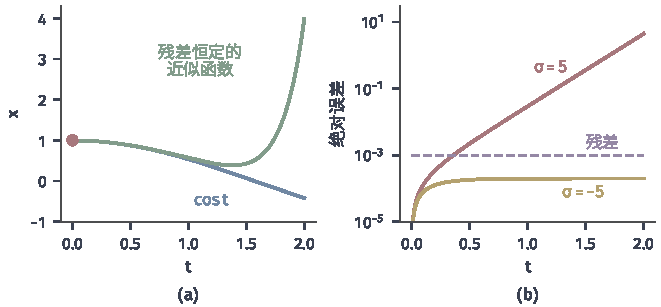
\includegraphics[width=112mm]{figures/06-differential-equations/01-ordinary-differential-equations/matplotlib/odenum-residual-gap/figure.pdf}
 \caption{残差相同而误差不同。(a)$\sigma=5$时，蓝线为真解$\cos t$，绿线为残差恒为$10^{-3}$的近似函数，二者很快分开。(b)绝对误差的对数图：紫色虚线是残差，红线和黄线分别是$\sigma=5$与$\sigma=-5$时的误差$\lvert d(t)\rvert$。}
 \label{fig:odenum-residual-gap}
\end{BookInlineFigure}

所以评价数值解时，要把初值误差、一步截断误差和每步计算误差分别记录，再结合误差的传播规律估计全局误差。这正是后面各节要做的事，传播规律由第~\ref{sec:odenum-error-convergence}节给出。

